\documentclass[math]{yanbook}

\usepackage{lipsum}
\usepackage{booktabs}
\usepackage{subcaption}
\usepackage{pgfplots}
\pgfplotsset{compat=1.18}
\usetikzlibrary{lindenmayersystems, decorations.pathmorphing, shapes, intersections, patterns}

\title{Yan Book}                 % 1. 标题
\subtitle{一个现代化的 LaTeX 模板} % 2. 副标题
\author{yaan}                    % 3. 作者
\institute{安徽大学}              % 4. 机构
\instituteen{Anhui University}   % 5. 机构英文
\date{\today}                    % 6. 日期
\version{1.0}                    % 7. 版本号
\location{于枫园}          % 8. 位置

\coverabstract{
    \qquad{}一个 \LaTeX\ 书籍模板,受 \href{https://github.com/alexmingzhang/latex-notes-template}{amznotes} 风格启发,有多种环境和功能,适合写作技术类书籍和文档。
    \par % 强制换段
    \qquad{}中文字体使用 \href{https://github.com/lxgw/LxgwWenKai}{LXGW WenKai},英文和数学字体使用 \href{https://github.com/alerque/libertinus}{libertinus},请你自行下载并安装。
}


\begin{document}

\makeatletter
\begin{titlepage}
        \newgeometry{margin=0pt}
        \thispagestyle{empty}
        \begin{tikzpicture}[remember picture, overlay]
            % --- 背景 ---
            \coordinate (split top) at ($(current page.north west)!0.7!(current page.north east)$);
            \shade[left color=yancovercolor!80!black, right color=yancovercolor!80!white, shading angle=90] 
                (split top) rectangle (current page.south east);
            
            % --- 右侧装饰诗句 (保留原样作为装饰,不再暴露配置,如需修改可在此处硬改) ---
            \node[anchor=center] at ($(split top)!0.5!(current page.south east)$) {
                \ifx\kaishu\undefined\newCJKfontfamily\kaishu{KaiTi}\fi
                \fontsize{24}{40}\selectfont \kaishu \color{white}
                \begin{tabular}{@{}c@{\hspace{1em}}c@{}}
                    一 & 月 \\ 只 & 亮 \\ 猫 & 想 \\ 吃 & 着 \\ 了 & 我 \\ 我 & 的 \\ 的 & 心 \\ 奶 & 事 \\ 酪 &
                \end{tabular}
            };
            
            % --- 左侧白底面板 ---
            \node[fill=white, anchor=north west, minimum height=\paperheight, minimum width=0.7\paperwidth, inner sep=0pt] 
                at (current page.north west) (leftpanel) {};
            
            % --- 左侧文字内容 ---
            \node[anchor=north west, inner sep=2cm, text width=0.55\paperwidth] at (leftpanel.north west) {
                \vspace{3cm}

                % === 标题区域 ===
                % 主标题
                {\fontsize{42}{50}\selectfont \sffamily \bfseries \textcolor{black!85}{\@title}}
                \\[0.2em] % 这里控制主标题和副标题的距离,0.2em 表示很近
                {\fontsize{16}{24}\selectfont \sffamily \textcolor{gray}{\@subtitle}}
                \\[2.5cm] % 这里控制副标题和下方装饰线的距离

                % 装饰线
                {\color{amzchaptercolor}\rule{2cm}{4pt}}\\[2.5cm]
                
                % 固定摘要 (可在此处修改固定文案)
                % {\sffamily \large \color{black!70} \setstretch{1.4}
                % \qquad{}本模板专注于\textbf{简洁}与\textbf{优雅}。
                % 灵感来源于现代界面设计,它拥有充足的留白、
                % 清晰的排版以及结构化的布局。
                % \par}\vspace{3cm}
                
                {\sffamily \large \color{black!70} \setstretch{1.4}
                \csname @coverabstract\endcsname
                \par}\vspace{3cm}




                % 底部信息表格 (使用你设置的变量)
                \noindent
                \begin{tabular}{@{} p{0.45\linewidth} p{0.45\linewidth} @{}}
                    {\sffamily \bfseries \footnotesize \textcolor{gray}{作者}} & {\sffamily \bfseries \footnotesize \textcolor{gray}{发布日期}} \\[0.5em]
                    {\sffamily \large \textbf{\@author}} & {\sffamily \large \textbf{\@date}} \\[0.8em]
                    
                    {\sffamily \bfseries \footnotesize \textcolor{gray}{机构}} & {\sffamily \bfseries \footnotesize \textcolor{gray}{版本}} \\[0.5em]
                    {\sffamily \small \textcolor{black!80}{\@institute}} & {\sffamily \small \textcolor{black!80}{\@version}} \\[0.1em]
                    {\sffamily \small \textcolor{black!40}{\@instituteen,\@location}} & {} 
                \end{tabular}
            };
            
            % --- Logo ---
            \node[anchor=north east, xshift=-2cm, yshift=-2cm] at (leftpanel.north east) {
                \begin{tikzpicture}
                    \fill[amzchaptercolor!20] (0,0) circle (0.8cm);
                    \fill[amzchaptercolor] (0.4,0.4) circle (0.3cm);
                \end{tikzpicture}
            };
        \end{tikzpicture}
        \restoregeometry
    \end{titlepage}
\makeatother

\tableofcontents
\printnomenclature[2cm]

\chapter{简介}
\epigraph{Mathematics is the queen of the sciences.}{Carl Friedrich Gauss}

\section{欢迎}

这是一个使用 \texttt{yanbook} 文档类的示例文档。

\begin{dfnbox}[Yanbook]{yanbook}
    \dfntxt{Yanbook} 是一个基于 \texttt{amznotes} 的自定义 LaTeX 文档类。
\end{dfnbox}

\begin{thmbox}[示理定理]{sample}
    这是一个定理盒子。
    \[ E = mc^2 \]
\end{thmbox}



\section{中文空格处理}

在 LaTeX 中处理中文时,空格的处理方式可能会让人困惑。以下是几种在中文中添加空格的方法:

\subsection{基本空格处理}

在中文文本中,直接输入空格通常不会显示,因为 CJK 字符(中文、日文、韩文)的排版规则与西文不同。例如:

\begin{verbatim}
这是没有空格的中文句子。
\end{verbatim}

\subsection{使用特殊命令}

要插入空格,您可以使用以下方法:

\begin{enumerate}
    \item 使用 \verb|\ | 命令:这\ 里\ 有\ 空\ 格
    \item 使用 \verb|~| 命令:这里~有~不间断空格
    \item 使用 \verb|\hspace{}| 命令:这里\hspace{1cm}有指定宽度的空格
    \item 使用 \verb|\qquad| 或 \verb|\quad|:这里\quad 有\qquad 更大的空格
\end{enumerate}

\subsection{中英文混排的空格}

在中英文混排时,LaTeX 通常会自动处理空格:

\begin{verbatim}
这是一个包含 English 和 数字 123 的句子。
\end{verbatim}

\subsection{调整中文字符间距}

如果需要调整中文字符之间的间距,可以临时使用:

\begin{verbatim}
\begin{CJKspace}
这 里 每 个 字 之 间 会 有 空 格
\end{CJKspace}
\end{verbatim}

但请注意,这不是标准的中文排版方式,一般情况下不推荐使用。

\subsection{实用技巧}

\begin{itemize}
    \item 在需要强调分隔的地方,使用标点符号而非空格
    \item 使用引号、括号等标点符号来组织文本结构
    \item 在中英文混排时,适当在英文前后添加空格以提高可读性
\end{itemize}

\chapter{功能展示}
\section{数学环境}

我们可以使用标准的 LaTeX 数学环境。

行内公式:$E = mc^2$。

行间公式:
\[
    \int_{-\infty}^{\infty} e^{-x^2} \, dx = \sqrt{\pi}
\]

\begin{thmbox}[微积分基本定理]{ftc}
    设 $f$ 是定义在闭区间 $[a, b]$ 上的连续实值函数。设 $F$ 是定义在 $[a, b]$ 上的函数,对于所有 $x \in [a, b]$,有
    \[
        F(x) = \int_a^x f(t) \, dt
    \]
    则 $F$ 在 $[a, b]$ 上一致连续,在开区间 $(a, b)$ 上可导,并且对于所有 $x \in (a, b)$,有
    \[
        F'(x) = f(x)
    \]
\end{thmbox}

\begin{lembox}[夹逼定理]{squeeze}
    如果 $g(x) \leq f(x) \leq h(x)$ 且 $\lim_{x \to a} g(x) = \lim_{x \to a} h(x) = L$,那么 $\lim_{x \to a} f(x) = L$。
\end{lembox}

\section{文本块}

\begin{dfnbox}[极限的定义]{limit-def}
    设 $f$ 是定义在包含 $c$ 的开区间(可能除去 $c$ 点)上的函数,且 $L$ 是一个实数。语句
    \[
        \lim_{x \to c} f(x) = L
    \]
    意味着对于任意 $\epsilon > 0$,存在一个 $\delta > 0$,使得如果 $0 < |x - c| < \delta$,则 $|f(x) - L| < \epsilon$。
\end{dfnbox}

\begin{exbox}[计算示例]{ex1}
    计算 $x \to 2$ 时 $f(x) = x^2$ 的极限。
    
    \textit{解:} 因为 $f(x)$ 是连续的,我们直接代入数值:
    \[
        \lim_{x \to 2} x^2 = 2^2 = 4
    \]
\end{exbox}

\begin{tecbox}[分部积分法]{int-parts}
    分部积分公式为:
    \[
        \int u \, dv = uv - \int v \, du
    \]
    当被积函数是两个函数的乘积时非常有用。
\end{tecbox}

\begin{notebox}
    这是一个简单的提示框。用于强调重要信息或警告。
\end{notebox}

\begin{genbox}{通用信息}
    这是一个通用盒子。可用于任何需要与正文区分的内容。
\end{genbox}

\section{代码块}

由于 \texttt{code} 选项当前已禁用(需要 Python 和 Pygments),这里展示一个使用盒子包裹 \texttt{verbatim} 的模拟代码块。

\begin{tcolorbox}[colback=gray!10, colframe=gray!50, title=Python 示例]
\begin{verbatim}
def hello_world():
    print("Hello, World!")
    return True

if __name__ == "__main__":
    hello_world()
\end{verbatim}
\end{tcolorbox}

如果你在 \texttt{documentclass} 中启用了 \texttt{code} 选项,你可以使用 \texttt{amzcode} 环境进行语法高亮:

\begin{verbatim}
\begin{amzcode}{python}
def hello_world():
    print("Hello, World!")
\end{amzcode}
\end{verbatim}

\section{图片与子图}

\begin{figure}[htbp]
    \centering
    \begin{tikzpicture}
        \draw[fill=amzchaptercolor!20, draw=amzchaptercolor, thick] (0,0) circle (1.5cm);
        \node at (0,0) {\sffamily\bfseries 圆};
    \end{tikzpicture}
    \caption{使用 TikZ 绘制的示例图片}
    \label{fig:circle}
\end{figure}

我们也可以并排排列图片。

\begin{figure}[htbp]
    \centering
    \begin{subfigure}[b]{0.45\textwidth}
        \centering
        \begin{tikzpicture}
            \draw[fill=amzthmboxcolor!20, draw=amzthmboxcolor, thick] (0,0) rectangle (3,2);
            \node at (1.5,1) {A};
        \end{tikzpicture}
        \caption{子图 A}
        \label{fig:subA}
    \end{subfigure}
    \hfill
    \begin{subfigure}[b]{0.45\textwidth}
        \centering
        \begin{tikzpicture}
            \draw[fill=amzexboxcolor!20, draw=amzexboxcolor, thick] (0,0) -- (1.5,2) -- (3,0) -- cycle;
            \node at (1.5,0.7) {B};
        \end{tikzpicture}
        \caption{子图 B}
        \label{fig:subB}
    \end{subfigure}
    \caption{并排的两个子图}
    \label{fig:subfigures}
\end{figure}

\section{表格}

这是一个使用 \texttt{booktabs} 的专业三线表示例。

\begin{table}[htbp]
    \centering
    \caption{模型对比}
    \label{tab:comparison}
    \begin{tabular}{lcr}
        \toprule
        \textbf{模型} & \textbf{准确率} & \textbf{时间 (ms)} \\
        \midrule
        基准模型 & 85.4\% & 12.5 \\
        模型 A  & 88.2\% & 15.3 \\
        模型 B  & 91.7\% & 22.1 \\
        \bottomrule
    \end{tabular}
\end{table}

\section{高级 TikZ 示例}

\subsection{分形 (L-System)}

这是一个使用 Lindenmayer 系统生成的植物分形。

\begin{figure}[htbp]
    \centering
    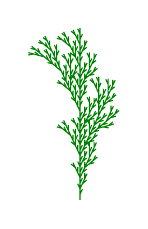
\begin{tikzpicture}
        \draw [green!50!black, rotate=90]
        [l-system={rule set={F -> F[-F]F[+F][F]}, axiom=F, order=4, step=2pt, angle=25}]
        l-system; 
    \end{tikzpicture}
    \caption{植物分形}
    \label{fig:fractal}
\end{figure}

\subsection{复变函数可视化}

这是一个使用 \texttt{pgfplots} 绘制的函数 $z = x e^{-x^2-y^2}$ 的 3D 图。

\begin{figure}[htbp]
    \centering
    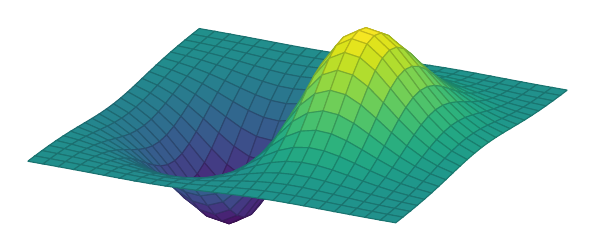
\begin{tikzpicture}
        \begin{axis}[
            colormap/viridis,
            hide axis,
        ]
        \addplot3[
            surf,
            domain=-2:2,
            domain y=-2:2,
        ]
        {exp(-x^2-y^2)*x};
        \end{axis}
    \end{tikzpicture}
    \caption{3D 曲面图}
    \label{fig:surface}
\end{figure}

\subsection{韦恩图}

表示三个集合 $A$、$B$ 和 $C$ 交集的韦恩图。

\begin{figure}[htbp]
    \centering
    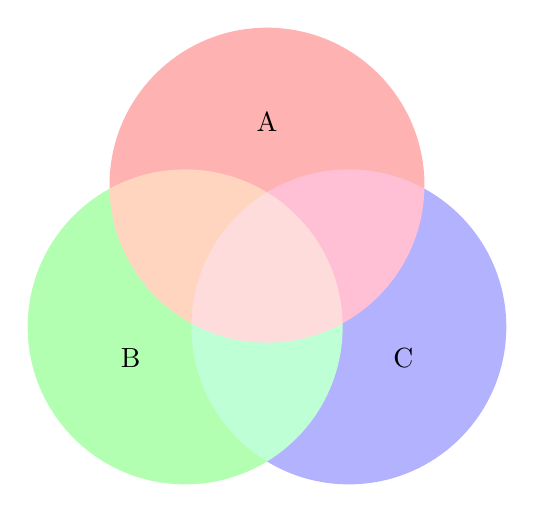
\begin{tikzpicture}
        \begin{scope}[blend group = soft light]
            \fill[red!30!white]   ( 90:1.2) circle (2);
            \fill[green!30!white] (210:1.2) circle (2);
            \fill[blue!30!white]  (330:1.2) circle (2);
        \end{scope}
        \node at ( 90:2)    {A};
        \node at ( 210:2)   {B};
        \node at ( 330:2)   {C};
    \end{tikzpicture}
    \caption{三个集合的韦恩图}
    \label{fig:venn}
\end{figure}

\section{对照块}

我们可以使用 \texttt{comparison} 环境并排对比两个概念。

\begin{comparison}
    \textbf{牛顿力学}
    
    \begin{itemize}
        \item 适用于宏观物体。
        \item 速度远小于光速。
        \item 空间和时间是绝对的。
        \item $F = ma$
    \end{itemize}
    
    \tcblower
    
    \textbf{相对论力学}
    
    \begin{itemize}
        \item 适用于所有速度。
        \item 接近光速时必须使用。
        \item 空间和时间是相对的。
        \item $E = mc^2$
    \end{itemize}
\end{comparison}

\section{Mac 风格代码块}

我们提供两种风格的代码块:浅色和深色。

\subsection{浅色模式}

\begin{maccode}[Python]{hello.py}
def factorial(n):
    """Calculates the factorial of n."""
    if n == 0:
        return 1
    else:
        return n * factorial(n-1)

print(factorial(5))
\end{maccode}

\subsection{深色模式}

\begin{macdarkcode}[C++]{main.cpp}
#include <iostream>

int main() {
    // This is a dark mode code block
    std::cout << "Hello, World!" << std::endl;
    return 0;
}
\end{macdarkcode}

\section{算法}

我们也可以精美地排版算法。

\begin{algobox}{欧几里得算法}
    \begin{algorithmic}[1]
        \Procedure{Euclid}{$a,b$} \Comment{a 和 b 的最大公约数}
            \State $r\gets a \bmod b$
            \While{$r\not=0$} \Comment{如果 r 为 0 则得到结果}
                \State $a \gets b$
                \State $b \gets r$
                \State $r \gets a \bmod b$
            \EndWhile\label{euclidendwhile}
            \State \textbf{return} $b$\Comment{最大公约数是 b}
        \EndProcedure
    \end{algorithmic}
\end{algobox}

\section{新功能:章节名言、术语表和全页图}

\epigraph{We must know. We will know.}{David Hilbert}

\subsection{术语表}
我们在这里定义一些符号。
\nomenclature{$c$}{真空惯性系中的光速}
\nomenclature{$h$}{普朗克常数}
\nomenclature{$G$}{万有引力常数}
\nomenclature{$\mathbb{R}$}{实数集}

符号 $c$、$h$ 和 $G$ 是基本常数。$\mathbb{R}$ 是一个集合。
请查看文档开头的术语表。

\subsection{全页背景}
下一页将有一个全页背景图(本例中使用 TikZ 模拟)。

\newpage
% Create a temporary pattern image for demonstration
\begin{tikzpicture}[remember picture, overlay]
    \node[opacity=0.1] at (current page.center) {
        \begin{tikzpicture}
            \foreach \i in {0,10,...,360}
                \draw [rotate=\i] (0,0) -- (0,15);
        \end{tikzpicture}
    };
    \node[font=\Huge\bfseries, text=red, rotate=45, opacity=0.3] at (current page.center) {背景示例};
\end{tikzpicture}
\fullpagebg[0.1]{example-image} % 实际使用时替换为图片路径


\chapter{基础使用指南}
\epigraph{The essence of mathematics lies in its freedom.}{Georg Cantor}

\section{项目结构}

\texttt{yanbook} 模板的组织结构如下:

\begin{itemize}
    \item \texttt{main.tex}: 主文档文件。
    \item \texttt{yanbook.cls}: 定义样式的自定义类文件。
    \item \texttt{Makefile}: 构建自动化脚本。
    \item \texttt{chapters/}: 包含章节内容文件的文件夹。
    \item \texttt{contents/}: 包含封面等其他内容的文件夹。
    \item \texttt{images/}: 用于存储图片的文件夹。
    \item \texttt{output/}: 生成的 PDF 存放目录。
    \item \texttt{build/}: 中间构建文件目录。
\end{itemize}

\section{编译}

本项目使用 \texttt{Makefile} 来简化编译过程。

\subsection{环境要求}
\begin{itemize}
    \item TeX 发行版 (TeX Live, MiKTeX, 或 MacTeX)
    \item XeLaTeX 引擎 (用于 Unicode 和字体支持)
    \item Make 工具 (可选但推荐)
\end{itemize}

\subsection{命令}
要编译项目,请在项目根目录打开终端并运行:

\begin{maccode}{bash}
make
\end{maccode}

该命令将:
\begin{enumerate}
    \item 使用 \texttt{xelatex} 编译文档。
    \item 运行 \texttt{biber} 处理参考文献 (如果需要)。
    \item 运行 \texttt{makeindex} 处理术语表。
    \item 重新编译以解决引用。
    \item 将最终的 PDF 移动到 \texttt{output/} 目录。
\end{enumerate}

清理构建文件:
\begin{maccode}{bash}
make clean
\end{maccode}

\section{文档类选项}

\texttt{yanbook} 类支持在 \texttt{main.tex} 中传递几个选项:

\begin{maccode}{latex}
\documentclass[math, code, fastcompile]{yanbook}
\end{maccode}

\begin{description}
    \item[math] 启用数学相关环境 (\texttt{thmbox}, \texttt{lembox}) 并加载 \texttt{mathtools}, \texttt{amsthm}, \texttt{derivative} 等宏包。
    \item[code] 启用 \texttt{minted} 宏包以进行高级代码高亮 (需要安装 Python 和 Pygments)。注意:模板也包含不需要此选项的独立 Mac 风格代码块。
    \item[fastcompile] 禁用一些耗时的样式功能 (如花哨的章节标题和部分盒子阴影) 以加快草稿阶段的编译速度。
\end{description}


\chapter{高级功能详解}
\section{文本盒子}

\epigraph{A mathematician is a machine for turning coffee into theorems.}{Paul Erdős}

模板提供了几种预定义的彩色盒子,用于不同类型的内容。

\subsection{定义与定理}

\begin{lstlisting}[language=TeX, frame=single]
\begin{dfnbox}[标题]{标签}
    内容...
\end{dfnbox}

\begin{thmbox}[标题]{标签}
    内容...
\end{thmbox}
\end{lstlisting}
也可以使用
\begin{lstlisting}[language=TeX, frame=single]
\begin{boxname*}{标题}
    有标题无记号
\end{boxname*}

\begin{boxname}{标题}
    无标题有记号
\end{boxname}

\end{lstlisting}
可用盒子:
\begin{itemize}
    \item \texttt{dfnbox}: 定义 (蓝色)
    \item \texttt{thmbox}: 定理 (紫色,需要 \texttt{math} 选项)
    \item \texttt{lembox}: 引理 (紫色,需要 \texttt{math} 选项)
    \item \texttt{exbox}: 示例 (黄色)
    \item \texttt{tecbox}: 技巧 (橙色)
    \item \texttt{genbox}: 通用信息 (绿色)
    \item \texttt{notebox}: 注意/警告 (红色,简单风格)
\end{itemize}

\section{代码块}

\subsection{Mac 风格窗口}
这些块模仿 macOS 窗口的外观。它们使用 \texttt{listings} 宏包,不需要 Python。

\textbf{浅色模式:}
\begin{lstlisting}[language=TeX, frame=single]
\begin{maccode}{python}
def hello():
    print("Hello")
\end{maccode}
\end{lstlisting}

\textbf{深色模式:}
\begin{lstlisting}[language=TeX, frame=single]
\begin{macdarkcode}{python}
def hello():
    print("Hello")
\end{macdarkcode}
\end{lstlisting}

\section{对照环境}

使用 \texttt{comparison} 环境并排显示两列内容,中间有垂直分隔线。

\begin{lstlisting}[language=TeX, frame=single]
\begin{comparison}
    左侧内容
    \tcblower
    右侧内容
\end{comparison}
\end{lstlisting}

\section{特殊功能}

\subsection{章节名言}
在章节开头添加名言:
\begin{lstlisting}[language=TeX, frame=single]
\epigraph{名言内容}{作者}
\end{lstlisting}

\subsection{术语表}
为术语表定义符号:
\begin{lstlisting}[language=TeX, frame=single]
\nomenclature{$x$}{x 的描述}
\end{lstlisting}
列表使用 \texttt{\textbackslash printnomenclature} 打印。

\subsection{全页背景}
在当前页面插入全页背景图片:
\begin{lstlisting}[language=TeX, frame=single]
\fullpagebg[0.5]{path/to/image.jpg}
\end{lstlisting}
可选参数控制不透明度 (默认为 1)。


\chapter{环境速览}
\section{环境速览}

本章展示本模板中可用的环境与其用法示例,便于快速参考与对照。

\subsection{盒子环境(tcolorbox)}

% dfnbox: 定义
\begin{dfnbox}[定义盒子示例]{defn-demo}
这是一个定义盒子,用于强调术语或关键定义。
\end{dfnbox}

% dfnbox*:仅标题版本
\begin{dfnbox*}{仅标题示例}
星号版本的盒子使用必填标题参数,无可选项。
\end{dfnbox*}

% exbox: 例子
\begin{exbox}[例子盒子示例]{ex-demo}
这是一个例子盒子,可用于演示具体案例或计算。
\end{exbox}

% tecbox: 技巧
\begin{tecbox}[技巧盒子示例]{tec-demo}
这是一个技巧盒子,用于记录解题技巧或方法提示。
\end{tecbox}

% genbox: 通用盒子(需要标题)
\begin{genbox}{通用盒子标题}
这是一个通用盒子,可自由放置内容与说明。
\end{genbox}

% notebox: 注记盒子
\begin{notebox}
这是一个注记盒子,适合放置提示、注意事项或小结。
\end{notebox}

% thmbox / lembox (仅 math 选项启用时可用)
\begin{thmbox}[定理盒子示例]{thm-demo}
若 $a>b$ 且 $b>c$,则 $a>c$。
\end{thmbox}

\begin{lembox}[引理盒子示例]{lem-demo}
若 $x>0$,则 $x^2\ge 0$。
\end{lembox}

\subsection{定理类环境(amsthm)}

\begin{theorem}
设 $x,y\in\mathbb{R}$。若 $x>y$,则对任意 $z\in\mathbb{R}$ 有 $x+z>y+z$。
\end{theorem}

\begin{lemma}
若 $x\ge 0$,则 $\sqrt{x}$ 存在且为非负数。
\end{lemma}

\begin{definition}
令函数 $f: A\to B$,若对任意 $x_1,x_2\in A$ 有 $x_1=x_2\Rightarrow f(x_1)=f(x_2)$,则称 $f$ 为良定义。
\end{definition}

\begin{proposition}
对任意 $x\in\mathbb{R}$,有 $|x|\ge 0$。
\end{proposition}

\begin{corollary}
若 $x\ne 0$,则 $x^2>0$。
\end{corollary}

\begin{remark}
本模板的定理环境按章节编号,并使用标准样式显示。
\end{remark}

\begin{example}
设 $f(x)=x^2$。则 $f'(x)=2x$。
\end{example}

\begin{problem}
求解 $x^2-1=0$ 的全部实数解。
\end{problem}

\begin{solution}
方程可因式分解为 $(x-1)(x+1)=0$,故解为 $x=\pm 1$。
\end{solution}

\begin{proof}
由加法保序性可知:若 $x>y$,则对任意 $z$,均有 $x+z>y+z$。证毕。
\end{proof}






\end{document}
